\chapter{Cahier des charges détaillé}
\label{chap:cdc_detaille}

Ce chapitre détaille les spécifications techniques du projet, en se basant sur les éléments imposés et l'architecture retenue. L'analyse est structurée autour des trois sous-systèmes principaux : l'alimentation (production et stockage), la distribution (consommation) et le monitoring (pilotage et supervision).

\section{Éléments imposés}

Le projet s'articule autour d'un ensemble de matériels et de contraintes techniques imposés, qui définissent le cadre de l'étude :

\begin{itemize}
    \item \textbf{Source d'alimentation renouvelable} : Alternateur d’éolienne.
    \item \textbf{Conversion de puissance} : Convertisseur MPPT pour l'optimisation de la charge batterie.
    \item \textbf{Stockage} : Batterie plomb/acide 48\,V - 200\,Ah.
    \item \textbf{Charges} :
    \begin{itemize}
        \item 4 points d’éclairage LED.
        \item Une prise USB standard (5\,V / 2\,A).
        \item Une prise USB-C Power Delivery (20\,V / 5\,A).
        \item Alimentation 24\,V pour le réfrigérateur.
        \item Alimentation modulable 450\,W pour le rice-cooker.
    \end{itemize}
    \item \textbf{Auxiliaires} : Alimentations stabilisées pour l'électronique de commande (15\,V, 5\,V, 3,3\,V).
    \item \textbf{Pilotage et Interface} : Instrumentation sur bus CAN et application web de gestion temps réel.
\end{itemize}

\section{Partie 1 : Alimentation et Stockage}

Cette première partie traite de la conversion de l'énergie mécanique du vent en énergie électrique stockable. Elle englobe la chaîne de conversion depuis l'alternateur jusqu'à la batterie 48\,V.

\subsection{Source d'énergie : L'éolienne simulée}

La source d’alimentation repose sur une simulation en laboratoire. Un moteur asynchrone entraîne l’alternateur pour reproduire le comportement mécanique des pales d’une éolienne soumise au vent. Cette configuration permet de reproduire différentes vitesses de vent et d’analyser le comportement du système dans des conditions variées et maîtrisées.

L’énergie mécanique produite par le moteur est transmise à un alternateur. Celui-ci assure la conversion de l’énergie mécanique en énergie électrique sous forme de courant alternatif (AC), conformément au principe de fonctionnement d’une éolienne réelle.
À la sortie de l’alternateur, un redresseur AC/DC est mis en œuvre afin de convertir le courant alternatif en courant continu (DC). Cette étape est indispensable pour obtenir une tension continue exploitable, notamment en vue du stockage de l’énergie dans une batterie.

L’ensemble constitue ainsi une plateforme expérimentale permettant d’étudier et d’optimiser le fonctionnement d’un système éolien dans un environnement contrôlé.

\subsubsection{Caractérisation de l’alternateur}

\paragraph{Essai à vide}
L'essai à vide permet de caractériser la force électromotrice de la machine sans débit de courant, c'est-à-dire sans charge connectée,  afin d’analyser son comportement intrinsèque. Il permet notamment d’étudier la relation entre la vitesse de rotation et la tension de sortie. Les relevés confirment la nature triphasée des tensions (déphasage de $2\pi/3$) et montrent une relation linéaire entre la vitesse de rotation et la tension efficace, caractéristique des machines synchrones.

Pour l’ensemble de nos mesures, nous considérons une plage de vitesses comprise entre 500 et 750 tr/min. Pour chaque vitesse, nous relevons la tension efficace et la fréquence en sortie de l’alternateur.

\begin{tableau}[H]
    \centering
    \begin{tabularx}{0.8\textwidth}{X X X}
        \toprule
        \textbf{Vitesse (tr/min)} & \textbf{Fréquence (Hz)} & \textbf{Tension efficace (V)} \\
        \midrule
        500 & 50,2 & 133 \\
        1000 & 101,6 & 245 \\
        1500 & 150,7 & 358 \\
        \bottomrule
    \end{tabularx}
    \caption{Résultats de l'essai à vide de l'alternateur}
    \label{tab:essai_a_vide}
\end{tableau}

Le nombre de paires de pôles $p$ est déduit de la fréquence $f$ et de la vitesse $N$ :
\begin{equation}
    p = \frac{60 \cdot f}{N} = \frac{60 \cdot 50}{500} = 6 \quad \text{paires de pôles}
\end{equation}

\paragraph{Essai en charge}
L'essai en charge, permet d'évaluer le comportement du générateur en puissance. La tension alternative produite par l’alternateur est redressée au moyen d’un pont de diodes afin d’obtenir une tension continue. Une charge de type RL, composée d’une résistance et d’une inductance, est ensuite connectée en sortie du redresseur pour reproduire des conditions de fonctionnement proches d’une utilisation réelle.

\begin{figure}[H]
    \centering
    \begin{tikzpicture}[scale=1.0, thick]

% Left vertical line connecting the phases
\draw (0,2) -- (0,-2);

% --- Top phase ---
\draw (0,2) -- (0.5,2);
% Source E
\draw (1,2) circle (0.5);
\draw (0.5,2) -- (1.5,2);
\node at (1, 2.8) {$E$};
\draw (1.5,2) -- (2,2);
% Inductor lambda
\draw (2,2) arc (180:0:0.2) arc (180:0:0.2) arc (180:0:0.2) arc (180:0:0.2);
\node at (2.8, 2.6) {$\lambda$};
\draw (3.6,2) -- (4,2);
% Resistor r
\draw (4, 1.6) rectangle (5.2, 2.4);
\node at (4.6, 2.8) {$r$};
\draw (5.2,2) -- (6,2);

% --- Middle phase ---
\draw (0,0) -- (0.5,0);
% Source
\draw (1,0) circle (0.5);
\draw (0.5,0) -- (1.5,0);
\draw (1.5,0) -- (2,0);
% Inductor
\draw (2,0) arc (180:0:0.2) arc (180:0:0.2) arc (180:0:0.2) arc (180:0:0.2);
\draw (3.6,0) -- (4,0);
% Resistor
\draw (4, -0.4) rectangle (5.2, 0.4);
\draw (5.2,0) -- (6,0);

% --- Bottom phase ---
\draw (0,-2) -- (0.5,-2);
% Source
\draw (1,-2) circle (0.5);
\draw (0.5,-2) -- (1.5,-2);
\draw (1.5,-2) -- (2,-2);
% Inductor
\draw (2,-2) arc (180:0:0.2) arc (180:0:0.2) arc (180:0:0.2) arc (180:0:0.2);
\draw (3.6,-2) -- (4,-2);
% Resistor
\draw (4, -2.4) rectangle (5.2, -1.6);
\draw (5.2,-2) -- (6,-2);

% --- Rectifier block ---
\draw (6,-3) rectangle (10,3);
\node at (8, 3.4) {\large Redresseur};
\node at (6.5, 2.2) {\Large $\sim$};
\node at (9.2, 2.2) {\large PD3};

% Diode inside
\draw (7.2, 0) -- (7.6, 0);
\draw (7.6, 0.4) -- (7.6, -0.4) -- (8.4, 0) -- cycle;
\draw (8.4, 0.4) -- (8.4, -0.4);
\draw (8.4, 0) -- (8.8, 0);

% --- Output side ---
\draw (10, 1.8) -- (12.5, 1.8);
\draw (10, -1.8) -- (12.5, -1.8);

% Voltage arrow
\draw[-{Stealth[length=3mm]}] (10.5, -1.5) -- (10.5, 1.5);
\node[right] at (10.5, 0) {$V_{CH}$};

% --- Load block ---
\draw[blue, thick] (11.5, -1.6) rectangle (13.5, 1.2);
\node[right, blue] at (13.8, 0) {\large Charge RL};

% Load components
\draw (12.5, 1.8) -- (12.5, 0.8);
% Variable resistor R
\draw (12.1, 0.2) rectangle (12.9, 0.8);
\draw[-{Stealth[length=2mm]}] (11.8, 0) -- (13.2, 1.0);
\node[right] at (12.9, 0.5) {$R$};
\draw (12.5, 0.2) -- (12.5, -0.2);
% Inductor L
\draw (12.5, -0.2) arc (90:-90:0.2) arc (90:-90:0.2) arc (90:-90:0.2);
\node[right] at (12.7, -0.8) {$L$};
\draw (12.5, -1.4) -- (12.5, -1.8);

\end{tikzpicture}
    \caption{Schéma du montage expérimental pour l'essai en charge de l'alternateur}
    \label{fig:montage_test_charge}
\end{figure}

Comme illustré précédemment, des résistances de \SI{330}{\ohm} ont été utilisées afin de simuler une seule phase de l’alternateur et de permettre la mesure de la tension aux bornes de cette phase.
Les valeurs efficaces des tensions et des courants sont mesurées aux bornes de l’alternateur (côté AC) et à la sortie du redresseur (côté DC), ainsi que la fréquence électrique pour différentes vitesses de rotation et différentes valeurs de la résistance de charge R.
La puissance quant à elle à été trouvée à l’aide de la fonction MATH sur l'oscilloscope à l'aide de la tension mesurée aux bornes de la charge et le courant mesuré à l’aide d'une pince ampèremétrique.
Les résultats obtenus sont présentés dans les figures suivantes :

% insertion des 3 scopes

\begin{figure}[H]
    \centering
    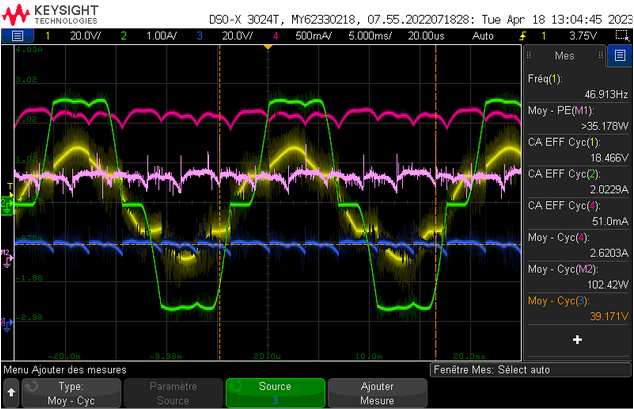
\includegraphics[width=0.8\textwidth]{images/scopes/Essai 500 trmin.png}
    \caption{Mesures à l’oscilloscope des grandeurs électriques de l’alternateur et du redresseur pour 500 tr/min}
    \label{fig:essai_500_trmin}
\end{figure}

\begin{figure}[H]
    \centering
    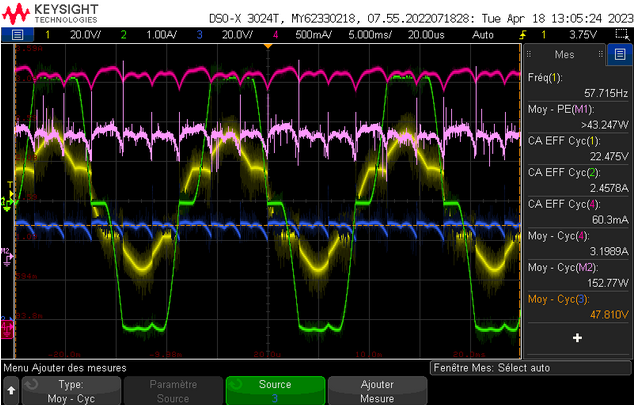
\includegraphics[width=0.8\textwidth]{images/scopes/Essai 600 trmin.png}
    \caption{Mesures à l’oscilloscope des grandeurs électriques de l’alternateur et du redresseur pour 600 tr/min}
    \label{fig:essai_600_trmin}
\end{figure}

\begin{figure}[H]
    \centering
    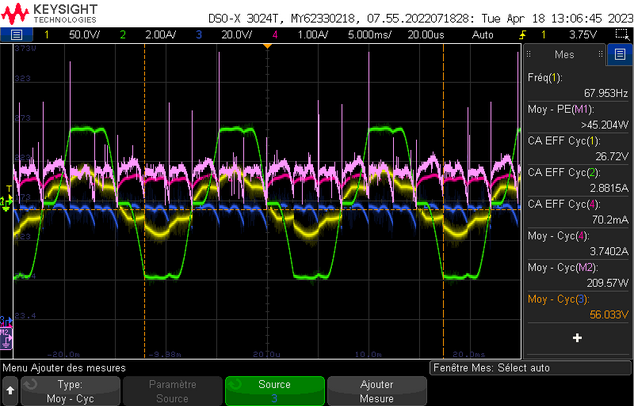
\includegraphics[width=0.8\textwidth]{images/scopes/Essai 700 trmin.png}
    \caption{Mesures à l’oscilloscope des grandeurs électriques de l’alternateur et du redresseur pour 700 tr/min}
    \label{fig:essai_700_trmin}
\end{figure}


Voici un résumé des résultats obtenus :

\begin{tableau}[H]
    \centering
    \begin{tabularx}{\textwidth}{X X X X X}
        \toprule
        \textbf{Vitesse (tr/min)} & \textbf{Fréq. (Hz)} & \textbf{Tension (V)} & \textbf{Courant (A)} & \textbf{Puissance (W)} \\
        \midrule
        500 & 46,9 & 39,2 & 2,62 & 102 \\
        600 & 57,7 & 47,8 & 3,20 & 153 \\
        700 & 67,9 & 56,0 & 3,74 & 210 \\
        \bottomrule
    \end{tabularx}
    \caption{Caractéristiques en charge après redressement}
    \label{tab:recap_charge}
\end{tableau}

Nous connaissons les caractéristiques  nominales de l’alternateur qui sont de 300W pour 750 tours/min, cependant lors de l’essai à 750 tr/min ce dernier n’a pas pu être mené à son terme. Sous charge, le moteur asynchrone d’entraînement ne parvenait pas à maintenir la vitesse nominale et calait immédiatement. Ce problème à empêché toute acquisition de mesures exploitables dans cette condition de fonctionnement.

\subsubsection{Modélisation de la source}
Pour concevoir le convertisseur MPPT, il est nécessaire de connaître l'impédance interne de la source (inductance de fuite). Celle-ci est déterminée en deux étapes à partir de l'observation de l'empiètement lors du redressement.

\paragraph{Calcul de l'empiètement}
L'empiètement $\mu$ est calculé à partir du temps de commutation des diodes observé à l'oscilloscope :
\begin{equation}
    \mu = 2 \cdot \pi \cdot f \cdot t_{com}
\end{equation}
où $f$ est la fréquence électrique et $t_{com}$ le temps de commutation.

\paragraph{Calcul de l'inductance interne}
À partir de l'empiètement $\mu$, l'inductance interne $\lambda$ est déduite à l'aide de la relation suivante :
\begin{equation}
    1 - \cos(\mu) = \frac{\lambda \cdot \omega \cdot I_{ch}}{V_s \cdot \sqrt{2} \cdot \sin(\pi/n)}
\end{equation}
D'où l'expression de l'inductance :
\begin{equation}
    \lambda = \frac{(1 - \cos\mu) \cdot V_s \cdot \sqrt{2} \cdot \sin(\pi/n)}{\omega \cdot I_{ch}}
\end{equation}

\textit{Note : Des mesures complémentaires sur oscilloscope sont encore nécessaires pour valider précisément le temps de commutation $t_{com}$ et finaliser la caractérisation de la source d’alimentation.}

\subsection{Convertisseur AC/DC (Redresseur)}
L'alternateur fournit en sortie une tension alternative, alors que le système nécessite une tension continue. Les redresseurs, qui assurent la transformation de l'énergie alternative en énergie continue, constituent l'une des solutions les plus courantes parmi les convertisseurs statiques. Cette conversion est essentielle pour obtenir une source de tension continue à partir de l'alimentation alternative.

Il existe principalement deux grandes catégories de redresseurs : non commandés et commandés.

Le choix final du redresseur dépend de la caractérisation complète de la source d'énergie et de la charge, étape désormais achevée et fournissant toutes les données nécessaires. Une analyse fonctionnelle et une étude bibliographique permettront d'identifier puis de sélectionner les deux ou trois solutions les plus pertinentes, qui seront ensuite simulées pour en valider les performances. La solution retenue sera dimensionnée, testée et validée avant fabrication, assurant un convertisseur fiable et parfaitement adapté à l'application.

\subsection{Gestion de la batterie et MPPT}
\label{sec:gestion_batterie}

Le stockage de l'énergie est assuré par un parc de batteries 48\,V, agissant comme tampon entre la production intermittente et la consommation.

\subsubsection{Caractéristiques du parc batterie}
Pour permettre de dimensionner correctement chaque convertisseur, il est important de bien comprendre le fonctionnement du parc de batteries, et plus particulièrement l'évolution des niveaux de tension en fonction de l'état de charge.
Les premières mesures réalisées au voltmètre aux bornes de chaque batterie au repos ont révélé des tensions aux alentours de 12,2\,V. En mettant ces 4 batteries en série, une tension réelle d'environ 48,8\,V est obtenue.
Le parc est donc constitué de 4 batteries 12\,V Plomb/Acide (200\,Ah) en série. Pour la suite du projet, il est crucial de garder à l'esprit que l'appellation « 48\,V » n'est qu'une valeur nominale. En pratique, la tension réelle varie significativement selon l'état de charge (SoC en anglais, pour State Of Charge) et le régime de fonctionnement, ce qui implique que tout le matériel connecté devra s'y adapter. Voici les principaux comportements à anticiper :

\begin{itemize}
    \item \textbf{La tension maximale lors de la recharge} : Pour “forcer” l'énergie à entrer dans une batterie, le chargeur doit appliquer une tension supérieure à la tension naturelle de celle-ci. Une batterie de 12\,V est composée de 6 cellules internes. Si une cellule pleine au repos délivre environ 2,1\,V ($6 \times 2,1 = 12,6\,\text{V}$), la chimie du plomb exige d'appliquer une tension d'environ 2,4\,V par cellule pour la recharger efficacement. Mathématiquement, la tension de charge atteint donc $6 \times 2,4 = 14,4\,\text{V}$ par batterie. Pour le parc de 4 éléments en série, la tension globale s'élève à $4 \times 14,4 = 57,6\,\text{V}$. Les convertisseurs devront impérativement être capables de supporter cette hausse (jusqu'à près de 58\,V) sans dommage.
    \item \textbf{La tension minimale de sécurité} : À l'inverse, pour éviter une dégradation irréversible des batteries (décharge profonde), le système de contrôle global devra couper l'alimentation vers les convertisseurs si la tension chute de manière critique (en dessous des seuils de sécurité indiqués dans le tableau ci-dessous).
    \item \textbf{La chute de tension en utilisation (sous charge)} : Il est important de ne pas confondre une batterie « en charge » et une batterie « sous charge » (qui alimente le système). Dès l'allumage de l'ensemble des équipements électriques, l'effort demandé fait artificiellement chuter la tension mesurée aux bornes des batteries en raison de leur résistance interne. Lors de la programmation, il faudra bien distinguer cette baisse de tension normale liée à l'utilisation d'une véritable batterie déchargée. Le système devra toutefois être capable d'estimer le niveau d'énergie restant en temps réel à partir des valeurs de référence suivantes.
\end{itemize}

\begin{tableau}[H]
    \centering
    \begin{tabularx}{\textwidth}{X l l X}
        \toprule
        \textbf{État de charge} & \textbf{Tension (12\,V)} & \textbf{Tension (48\,V)} & \textbf{État de la batterie} \\
        \midrule
        100\% & 12,6\,V - 12,7\,V & 50,4\,V - 50,8\,V & Charge complète \\
        80\% & 12,4\,V & 49,6\,V & Bon état \\
        60\% & 12,2\,V & 48,8\,V & Partiellement déchargée \\
        40\% & 11,9\,V & 47,6\,V & Décharge critique \\
        20\% & 11,6\,V & 46,4\,V & Décharge profonde (Dégâts matériels) \\
        10\% ou moins & 11,3\,V ou moins & 45,2\,V ou moins & Batterie potentiellement hors d’usage \\
        \bottomrule
    \end{tabularx}
    \caption{État de charge des batteries en fonction de la tension à vide}
    \label{tab:batterie_soc_new}
\end{tableau}

\subsubsection{Convertisseur DC/DC et Stratégie MPPT}

Étant donné que la tension continue issue du pont redresseur varie fortement en fonction de la vitesse de rotation de l’alternateur (elle-même dépendante des fluctuations du vent simulé), il est indispensable d’intégrer un convertisseur DC/DC commandé par un algorithme MPPT. Le MPPT, de l'anglais Maximum Power Point Tracking, a pour objectif de maximiser en permanence la puissance extraite de la source, en s’assurant que le système fonctionne toujours au point de puissance maximal. \\
Ce convertisseur a un double rôle : Adapter dynamiquement l’impédance vue par l’alternateur afin d’extraire la puissance maximale disponible et convertir la tension redressée variable en une tension compatible avec la charge d’une batterie 48 V.

\section{Partie 2 : Distribution et Charges}
\label{sec:distribution}

Cette partie détaille l'ensemble des équipements connectés au bus 48\,V. Chaque charge nécessite une interface de puissance spécifique pour adapter la tension du bus aux besoins de l'application.

\subsection{Électroménager de puissance : Le Rice Cooker}
\label{subsec:rice_cooker}

L'intégration du rice-cooker au système nécessite une adaptation profonde de son alimentation d'origine afin de respecter les contraintes de puissance et de nature du réseau.

\subsubsection{Objectif d'adaptation et ergonomie}
L'objectif est de garantir une utilisation « transparente » pour l'utilisateur final. L'appareil, initialement conçu pour fonctionner en courant alternatif (230\,V$_{ac}$), doit être modifié pour s'intégrer à l'installation en courant continu. Il convient donc de s'assurer que l'ensemble des composants internes peuvent fonctionner sous la tension continue prévue sans dégradation de leurs fonctions.

\subsubsection{Caractéristiques techniques de la charge}
Les spécifications retenues pour le rice-cooker au sein du projet sont les suivantes :
\begin{itemize}
    \item \textbf{Puissance de fonctionnement} : Limitée à 450\,W (contre 700\,W d'origine).
    \item \textbf{Nature de la charge} : Charge majoritairement résistive avec une composante inductive mineure.
    \item \textbf{Mesures d'impédance} : Une caractérisation au RLCmètre à 10\,kHz a permis de mesurer une résistance $R = 78\,\Omega$ et une inductance $L \approx 10-11\,\mu$H.
    \item \textbf{Modulation de puissance} : L'alimentation doit être modulable afin de faire varier la puissance de chauffe selon le mode désiré (cuisson et maintien en température).
    \item \textbf{Adaptation} : Fonctionnement en tension continue au lieu d’une tension alternative provenant du réseau domestique (230\,V$_{ac}$).

\end{itemize}

\subsubsection{Alimentation du Rice Cooker}
Le rice-cooker est un équipement qui permet de faire cuire du riz à l’aide d’une résistance de qui va dissiper de la chaleur par effet Joule lors du passage d’un courant. C’est un équipement énergivore donc on a limité sa puissance à 450\,W. Son alimentation à partir du bus 48\,V, va nécessiter la création d’un convertisseur élévateur de tension continu (hacheur).
En considérant une tension d'entrée nominale $V_e = 50$\,V et une puissance de sortie maximale $P_s = 450$\,W, les grandeurs électriques sont déterminées comme suit :

Le courant de sortie requis pour la charge est de :
\begin{equation}
    I_s = \sqrt{\frac{P_s}{R}} = \sqrt{\frac{450}{78}} \approx 2,40\,\text{A}
\end{equation}

La tension de sortie du convertisseur doit donc être de :
\begin{equation}
    V_s = \frac{P_s}{I_s} = \frac{450}{2,40} = 187,5\,\text{V}
\end{equation}

Le gain en tension statique $G$ du convertisseur est alors :
\begin{equation}
    G = \frac{V_s}{V_e} = \frac{187,5}{50} = 3,75
\end{equation}

Sous l'hypothèse d'une conservation de la puissance active (en négligeant les pertes du convertisseur), la puissance d'entrée $P_e$ est égale à $P_s = 450$\,W. Le courant d'entrée moyen $I_e$ est alors :
\begin{equation}
    I_e = \frac{V_s \cdot I_s}{V_e} = \frac{187,5 \cdot 2,40}{50} = 9\,\text{A}
\end{equation}

En pratique, il convient de prévoir une marge de puissance supplémentaire pour compenser les pertes de conduction et de commutation du hacheur. Les composants de puissance et la structure du hacheur devront être dimensionnés pour supporter ces contraintes de courant (9\,A à l'entrée) et de tension (187,5\,V à la sortie).

\paragraph{Synthèse des caractéristiques techniques du hacheur}

Sur la base des calculs précédents, les spécifications techniques du convertisseur élévateur sont résumées comme suit :
\begin{itemize}
    \item \textbf{Grandeurs d'entrée} : environ 50\,V$_{dc}$ / 9\,A. Cette tension peut être légèrement plus élevée lorsque les batteries Plomb/Acide sont en fin de charge (jusqu'à 58\,V).
    \item \textbf{Grandeurs de sortie} : environ 187,5\,V$_{dc}$ / 2,40\,A.
\end{itemize}

\subsection{Éclairage domestique}

% insère une phrase d'introduction pour présenter le contexte de l'éclairage domestique dans la maquette et les besoins spécifiques liés à l'échelle réduite.


\subsubsection{Fonctions globales}
\begin{itemize}
    \item Adapter la tension de la batterie (48\,V) aux besoins spécifiques du réseau d'éclairage.
    \item Distribuer l'énergie vers les 4 points d'éclairage LED définis (Cuisine, Salon, Coin lecture, Toilettes).
    \item Permettre l'allumage et l'extinction de chaque zone d'éclairage de façon manuelle et indépendante.
    \item Protéger matériellement les circuits d'éclairage contre les surintensités.
\end{itemize}

\subsubsection{Conversion d'énergie pour l'éclairage}
Le système doit être capable de transformer la tension continue issue de la batterie de stockage principale (plage de 42\,V à 58\,V) en une tension stable et sécurisée pour les luminaires de la maquette. Pour cela nous devons mettre en place :
\begin{itemize}
    \item Un convertisseur DC/DC industriel du commerce abaissant la tension de la batterie (48\,V) vers un réseau 24\,V DC.
    \item Un dimensionnement optimisé pour une consommation totale inférieure à 20\,W. Ces puissances sont volontairement adaptées à l'échelle réduite de la maquette : elles suffisent amplement à reproduire les niveaux d'éclairement normés d'une vraie maison (en Lux) sans provoquer d'éblouissement sur une surface miniature. La puissance est répartie de la manière suivante selon le besoin lumineux des pièces :
    \begin{itemize}
        \item \textbf{Cuisine} : $\approx 6$\,W (Éclairage de travail fort).
        \item \textbf{Salon} : $\approx 5$\,W (Éclairage d'ambiance moyen).
        \item \textbf{Toilettes} : $\approx 3$\,W.
        \item \textbf{Coin lecture} : $\approx 2$\,W (Éclairage minimal).
    \end{itemize}
    (Total estimé : $\approx 16$\,W, ce qui laisse une marge de sécurité technique pour le convertisseur).
\end{itemize}

\subsubsection{Distribution et commande de l'éclairage}
L'installation doit permettre un contrôle simple et direct par l'utilisateur. Ainsi le circuit de distribution doit comporter :
\begin{itemize}
    \item Des interrupteurs mécaniques classiques placés sur chaque ligne pour contrôler les 4 zones séparément.
\end{itemize}

\subsection{Réfrigérateur}

\subsubsection{Fonctions globales}
\begin{itemize}
    \item Alimenter le réfrigérateur à partir du réseau de distribution continu adapté (24\,V).
    \item Assurer la production de froid de manière autonome.
\end{itemize}

\subsubsection{Caractéristiques de l'équipement}
D'après la plaque signalétique du réfrigérateur, les spécifications électriques requises sont :
\begin{itemize}
    \item \textbf{Tension d'entrée} : 12/24\,V$_{dc}$.
    \item \textbf{Puissance nominale} : 42\,W.
\end{itemize}

\subsubsection{Tests et analyse de consommation}
Afin de valider le comportement électrique réel du compresseur sous 24\,V, nous avons effectué des mesures de courant :
\begin{itemize}
    \item \textbf{Régime transitoire (Démarrage)} : Lors de la mise en route, on relève un appel de courant générant un pic à 8\,A maximum.
    \item \textbf{Régime permanent} : Une fois la vitesse du compresseur stabilisée, la consommation mesurée en continu s'établit à 1,4\,A.
\end{itemize}

\begin{figure}[H]
    \centering
    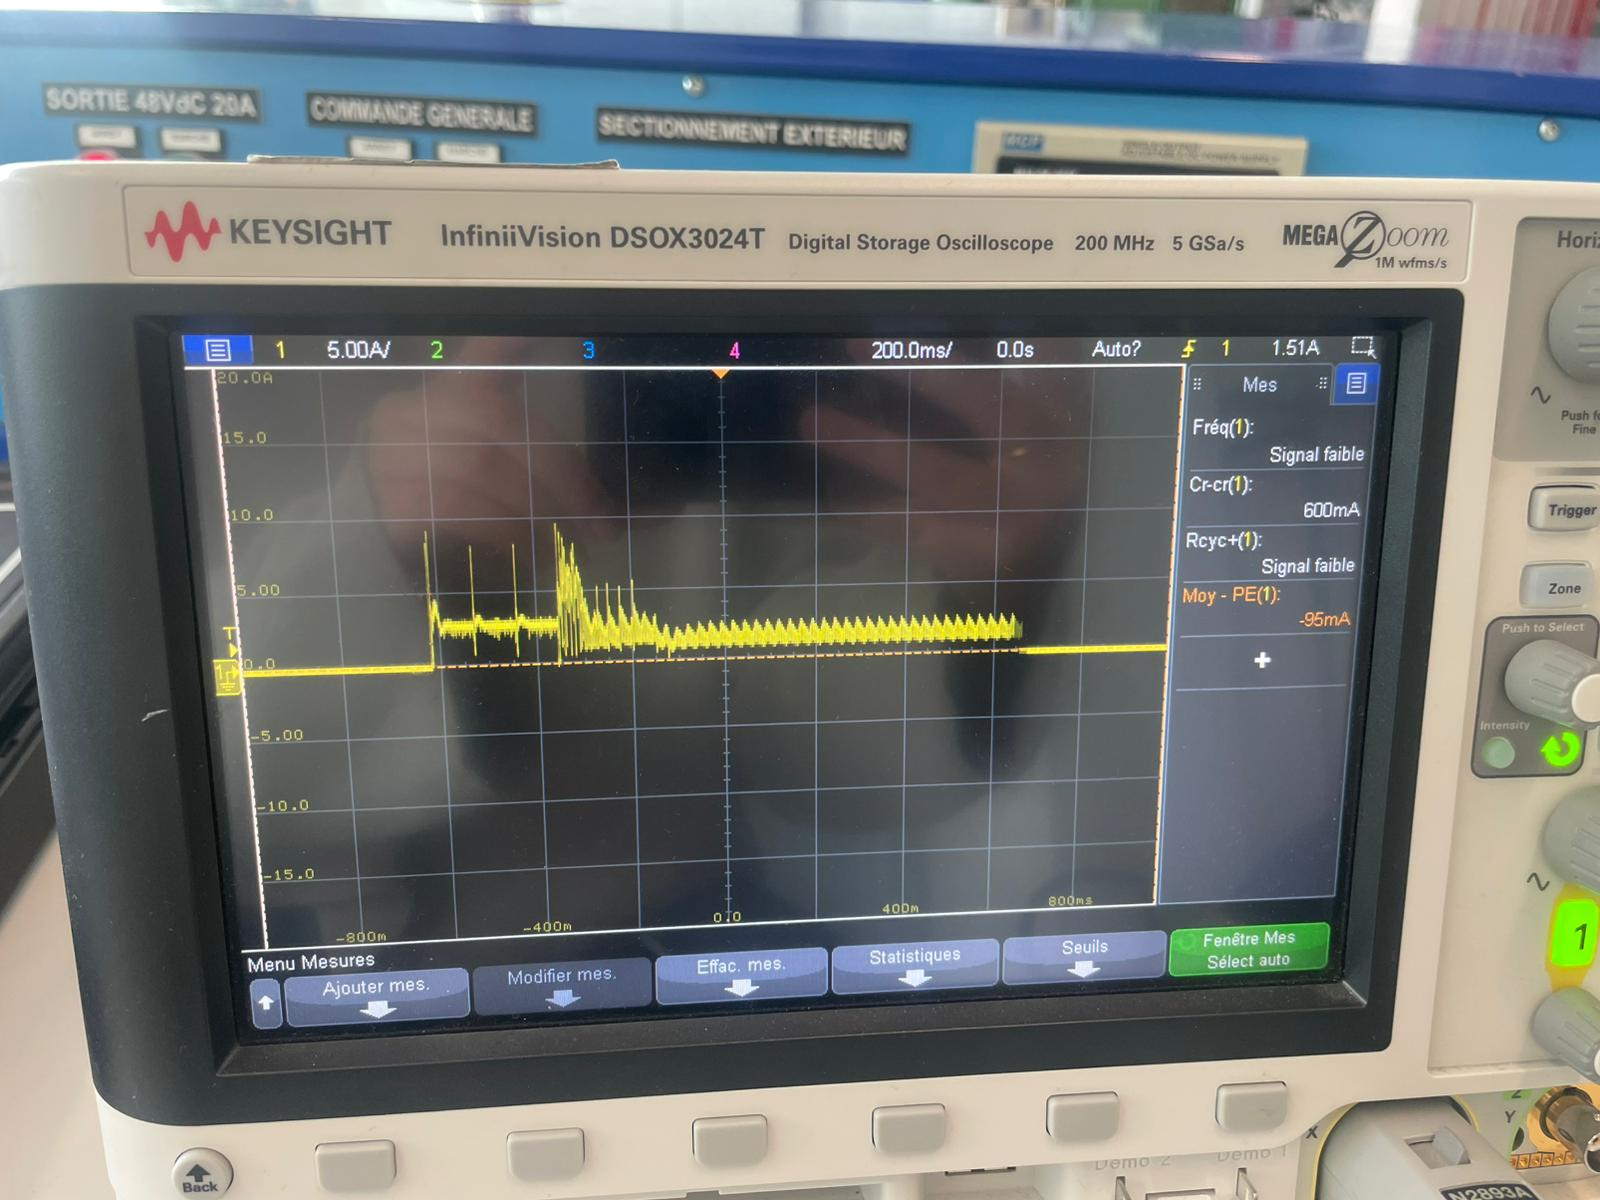
\includegraphics[width=0.8\textwidth]{images/scopes/scope refrigerateur.jpeg}
    \caption{Mesure à l’oscilloscope du courant de démarrage du réfrigérateur}
    \label{fig:scope_refrigerateur}
\end{figure}

Les protections devront être adaptées pour permettre au réfrigérateur de démarrer sans déclencher l’ouverture de son circuit d'alimentation.

\subsection{Distribution USB (Multimédia)}

L’intégration de ports USB au sein du système permet d’alimenter des équipements électroniques basse tension à partir du bus batterie 48\,V.
Aujourd’hui, les standards USB-B et USB-C sont devenus incontournables dans l’alimentation des dispositifs électroniques, qu’il s’agisse de périphériques classiques (5\,V) ou d’équipements nécessitant une puissance plus élevée via la norme USB-C Power Delivery (20\,V / 5\,A).

L’objectif de cette partie est donc d’assurer une conversion d’énergie fiable, efficace et sécurisée, tout en garantissant la compatibilité avec les normes électriques en vigueur.
La tension issue du pack batterie est nominalement de 48\,V, mais elle varie selon l’état de charge :
\begin{itemize}
    \item En fin de décharge $\approx 42$\,V
    \item En charge maximale $\approx 58$\,V
\end{itemize}
Les convertisseurs devront donc fonctionner correctement sur toute cette plage de tension.

La distribution USB doit répondre aux exigences suivantes :
\begin{itemize}
    \item Adapter la tension 48\,V aux niveaux requis par les normes USB (5\,V et 20\,V)
    \item Fournir une tension régulée avec une faible ondulation
    \item Garantir la protection contre les surtensions, surintensités et courts-circuits
    \item Permettre la mesure du courant et de la tension pour la partie monitoring
    \item Autoriser le délestage du port USB-C en cas de batterie faible afin de préserver l’autonomie du système
    \item Assurer un bon rendement énergétique pour limiter les pertes et l’échauffement
\end{itemize}
Cette architecture permet d’alimenter à la fois les dispositifs externes (prises USB) et certains systèmes internes de commande (Raspberry Pi, microcontrôleurs), tout en conservant une gestion centralisée de l’énergie.

\subsubsection{USB-B (5\,V / 7\,A)}
\paragraph{Caractéristiques et contraintes}
\begin{itemize}
    \item \textbf{Tension d’entrée} : 42\,V à 58\,V
    \item \textbf{Tension de sortie régulée} : 5\,V$_{dc}$
    \item \textbf{Tolérance} : conforme à la norme USB ($\pm 5\,\%$)
    \item \textbf{Courant nominal minimal} : 2\,A + 5\,A (Alimentation de la partie monitoring)
    \item \textbf{Puissance maximale estimée} : 35\,W
    \item \textbf{Stabilité} : Faible ondulation de sortie afin de garantir la stabilité des équipements électroniques sensibles
    \item \textbf{Protection contre} : les surtensions, les surintensités, les courts-circuits
    \item \textbf{Intégration} : dans l’architecture globale du système (montage industriel)
    \item \textbf{Supervision} : Possibilité de mesurer courant et tension pour le monitoring
\end{itemize}

\paragraph{Principe de conversion}
La tension du bus batterie (48\,V nominal) étant supérieure à la tension requise en sortie (5\,V), une conversion DC-DC abaisseuse est nécessaire afin d’adapter le niveau de tension tout en garantissant un bon rendement énergétique.
Un schéma bloc de la chaîne d’énergie est présenté ci-dessous :

\begin{figure}[H]
    \centering
    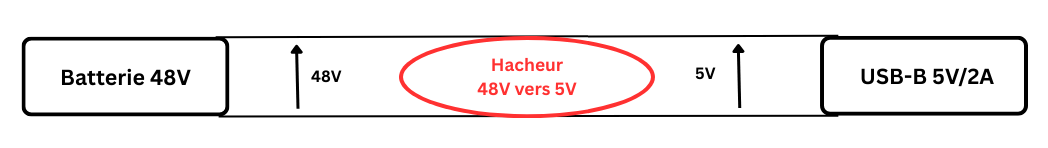
\includegraphics[width=0.8\textwidth]{images/figures/USB-B.png}
\end{figure}


\subsubsection{USB-C (20\,V / 5\,A)}
\paragraph{Caractéristiques et contraintes}
\begin{itemize}
    \item \textbf{Tension d’entrée} : 42\,V à 58\,V
    \item \textbf{Tension de sortie} : 20\,V$_{dc}$
    \item \textbf{Courant maximal} : 5\,A
    \item \textbf{Puissance maximale} : 100\,W
\end{itemize}
Les contraintes relatives à la stabilité de la tension, à la limitation d’ondulation, aux protections électriques (surtension, surintensité, court-circuit), à l’intégration mécanique ainsi qu’à la supervision énergétique sont identiques à celles décrites pour le convertisseur USB-B.

\paragraph{Principe de conversion}
Comme pour le port USB-B, l’adaptation de la tension du bus batterie vers la tension requise en sortie nécessite une conversion DC-DC abaisseuse. La chaîne d’énergie est donc la suivante :

\begin{figure}[H]
    \centering
    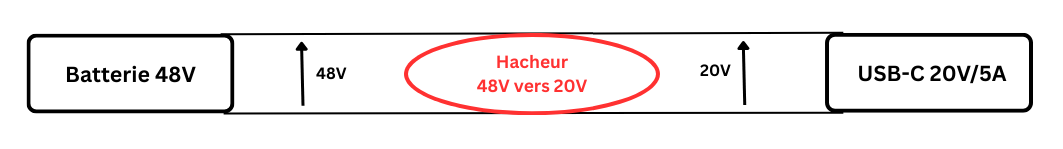
\includegraphics[width=0.8\textwidth]{images/figures/USB-C.png}
\end{figure}

\section{Partie 3 : Monitoring et Contrôle}
\label{sec:monitoring}

Le système de contrôle est le "cerveau" de l'installation. Il assure la sécurité, la gestion de l'énergie et l'interface utilisateur.
Afin de pouvoir contrôler, monitorer et réguler l’ensemble de l’installation, il est fondamental de pouvoir mesurer avec précision les grandeurs électriques (tension et courant) à des points clés du circuit. Ces données sont cruciales pour calculer la puissance produite par l’éolienne, la consommation de chaque équipement et l'état de charge de la batterie, permettant ainsi d’assurer le pilotage intelligent du système et le délestage des charges si nécessaire.

\subsection{Instrumentation - Relevé des grandeurs électriques du système}
Le système doit être capable de connaître différentes valeurs de courant et tension en temps réel, et cela pour chaque équipement de l’installation électrique. Pour cela nous devons mettre en place pour chaque convertisseur : 
\begin{itemize}
    \item Un dispositif permettant de capter un niveau de courant.
    \item Un dispositif permettant de capter un niveau de tension.
\end{itemize}

Voici l'ordre de grandeur des valeurs électriques que nous aurons à mesurer (données de dimensionnement des capteurs) : 

\begin{tableau}[H]
    \centering
    \begin{tabularx}{\textwidth}{X c c}
        \toprule
        \textbf{Convertisseur} & \textbf{Courant attendu (A)} & \textbf{Tension attendue (V)} \\
        \midrule
        USB-B & 7 & 5 \\
        USB-C & 5 & 20 \\
        Rice-cooker amont & 9 & 50 \\
        Rice-cooker aval & 2,40 & 187,5 \\
        Réfrigérateur & 8 (pic) / 1,4 (stabilisé) & 24 \\
        Éclairage & 0,85 & 24 \\
        MPPT amont & ??? & ??? \\
        MPPT aval & ??? & 48 \\
        \bottomrule
    \end{tabularx}
    \caption{Ordres de grandeur des mesures pour le monitoring}
    \label{tab:monitoring_values_detailed}
\end{tableau}

\subsection{Architecture de communication}
Les composants programmables présents dans le système doivent-être en capacité de se transmettre des données. Il faut donc que chaque composant soit relié aux autres. Le pilotage est distribué : chaque sous-ensemble (convertisseurs, capteurs) communique via un bus de terrain \textbf{CAN (Controller Area Network)}. Ce choix garantit la robustesse des échanges dans un environnement électriquement bruité (hacheurs de puissance). Le système devra donc comporter une gestion des priorités de communication. Les données collectées sont ensuite centralisées et traitées par un microcontrôleur ou un mini-ordinateur (ex : Raspberry Pi) qui assure la supervision globale du système.

\subsection{Traitement et analyse des données}
Le système doit pouvoir traiter les données mesurées à chaque instant. Il doit être capable d’utiliser des valeurs de tension et courant pour déterminer : 
\begin{itemize}
    \item La puissance générée par l’éolienne.
    \item La consommation de chaque équipement.
    \item L’état de charge de la batterie.
    \item Le temps restant estimé d’utilisation par équipement.
\end{itemize}

\subsection{Stratégie de délestage}
Afin de protéger la batterie contre les décharges profondes, le système supervise la tension du bus 48\,V. En cas de baisse critique, un délestage automatique est opéré selon un ordre de priorité défini :
\begin{enumerate}
    \item Rice-cooker (arrêt immédiat).
    \item Port USB-C (coupure).
    \item Réfrigérateur.
\end{enumerate}
L'éclairage et le système de monitoring restent alimentés le plus longtemps possible.

\subsection{Interface Homme-Machine (IHM)}
Le système doit permettre à l’utilisateur de visualiser les données acquises via une interface web, soit depuis un écran directement sur le dispositif de contrôle, soit par l’intermédiaire de tout navigateur web connecté au réseau internet de l’environnement.
Une application web, hébergée localement, permet à l'utilisateur de visualiser l'état du système selon deux modes d’affichage :



\begin{itemize}
    \item Un mode d’affichage \textbf{simplifié} pour l'utilisateur lambda avec des informations sur la charge globale du système, la production d’énergie et si l’énergie disponible permet d’utiliser les différents équipements.
    \item Un mode d’affichage \textbf{expert} indiquant toutes les mesures effectuées (tensions, courants, etc…) permettant un contrôle plus fin sur le système.
\end{itemize}